\documentclass[11pt]{article}

\usepackage[T1]{fontenc}
\usepackage{babel}
\usepackage[a4paper, total={6in, 10in}]{geometry}

\usepackage{float}
\usepackage[usenames,dvipsnames]{xcolor}
\usepackage[most]{tcolorbox}
\usepackage{listings} % per scrittura di codice
\usepackage{algorithmic}
\usepackage{algorithm}
\usepackage{booktabs}
\usepackage{multirow}
\usepackage{hyperref}
\usepackage{graphicx}
\usepackage{subcaption}

\definecolor{verdeNEO4J}{RGB}{3, 140, 11}
\definecolor{celesteNEO4J}{RGB}{48, 119, 166}
\hypersetup{
    colorlinks=true,
    linkcolor=blue,
    filecolor=cyan,      
    urlcolor=magenta,
    pdftitle={Overleaf Example},
    pdfpagemode=FullScreen,
    }


\usepackage{graphicx}
\graphicspath{{./images}}

\definecolor{InlineGray}{HTML}{E3E3E3}
\lstset{numbers=left}

% this style should be active for all lstlistings environments
\lstdefinestyle{all}{
 tabsize=2,
 columns=fixed,
 keepspaces=true,
 frameshape={}{y}{}{}, % per rimuovere la linea vericale sulla sinistra `frameshape={}{}{}{}`
 basicstyle = {\ttfamily \color{black}},
 showstringspaces=false,
 rulecolor=\color{black},
 numberstyle=\tiny\color{black}
}

\lstdefinestyle{inline}{
 basicstyle={\small\ttfamily \color{black}},
 columns=fixed,
 showstringspaces=false,
}

\lstdefinestyle{PythonStyle}
{
 language=Python,
 breaklines=true,
 breakatwhitespace=true,
 stringstyle=\color{Bittersweet},
 commentstyle=\color{darkgray},
 keywordstyle=\color{violet},
 keywordstyle=[2]\color{violet},
 morekeywords=[2]{agg,avg,alias,sort,ascending,groupBy,withColumn,filter,join,withColumnRenamed,where,select,desc,drop,row_number,over}
}

\lstdefinestyle{CypherStyle}
{
 breaklines=true,
 breakatwhitespace=true,
 stringstyle=\color{red},
 commentstyle=\color{gray},
 keywordstyle=\color{violet},
 keywordstyle=[2]\color{celesteNEO4J},
 keywordstyle=[3]\color{verdeNEO4J},
 morekeywords=[2]{collect, round, size, count},
 morekeywords=[3]{MATCH, WITH, RETURN, UNWIND, SUM, WHERE, ORDER, BY, DESC, AS, COUNT, DISTINCT, AND, CALL, UNION, YIELD, OR}
}

\lstdefinestyle{ArangoStyle}
{
 breaklines=true,
 breakatwhitespace=true,
 stringstyle=\color{red},
 commentstyle=\color{gray},
 keywordstyle=\color{violet},
 keywordstyle=[2]\color{gray},
 keywordstyle=[3]\color{blue},
 morekeywords=[2]{LENGTH, SUM},
 morekeywords=[3]{LET, FOR, RETURN, COLLECT, SORT, FILTER, LIMIT, IN, OUTBOUND, INBOUND, WITH, COUNT, INTO, DESC, DISTINCT, AGGREGATE, AND}
}

\lstdefinestyle{GSQLStyle}
{
 breaklines=true,
 string = [d]{"},
 breakatwhitespace=true,
 stringstyle=\color{brown},
 commentstyle=\color{gray},
 keywordstyle=\color{violet},
 keywordstyle=[1]\color{brown},
 keywordstyle=[2]\color{blue},
 keywordstyle=[3]\color{celesteNEO4J},
 morekeywords=[1]{STRING, ListAccum, MapAccum, SetAccum, SumAccum, HeapAccum},
 morekeywords=[2]{RUN, CREATE, FOREACH, PRINT, ACCUM, QUERY, GRAPH, FROM, FOR, FOREACH, SELECT, TUPLE, INSTALL, DO, IN, TYPEDEF, END, IF, THEN, ELSE, WHERE, AS},
 morekeywords=[3]{VERTEX, EDGE, INT, STRRING, FLOAT, LONG}
}


\tcbset{on line, 
    boxsep=2pt, left=0pt,right=0pt,top=0pt,bottom=0pt,
    colframe=white,colback=InlineGray,
}
\newcommand{\codeinline}[1]{\tcbox{\lstinline[style=inline]|#1|}}

\author{
 Stefanelli Francesco \\
 Matricola 538549\\
 \texttt{fra.stefanelli3@stud.uniroma3.it}
 \and
 Galletti, Davide \\
 Matricola 533152\\
 \texttt{dav.galletti@stud.uniroma3.it}
}

\title{\huge\textbf{Report Secondo Progetto Big Data} \\ \Large Comparison of GDBMSs for data analysis on GitHub commit data }
\date{\textbf{Data Team} \\
\href{https://github.com/BD-Data-Team/second-project-bigdata}{GitHub: data-team}\\
Anno Accademico 2022/2023}



\begin{document}
\maketitle
In questa relazione è stato documentato il lavoro svolto durante lo sviluppo del secondo progetto del corso di Big Data.
La relazione si divide in quattro sezioni: nella prima sezione viene riporato l'obiettivo del progetto; nella seconda viene presentato il dataset e lo schema a grafo impiegato; nella terza l'architettura big data e le tecnologie scelte; infine vengono analizzate le diverse soluzioni dei GDBMS secondo differenti scenari, andando a trarre delle conclusioni.


\section{Obiettivo}
L'obiettivo del progetto è quello di mettere a confronto tre diversi \textbf{GDBMS} dal punto di vista di \textbf{usabilità} e \textbf{prestazioni} in un contesto Big Data, dove il volume dei dati cresce nel tempo. A tale scopo sono stati definiti diversi scenari di analisi (query complesse e tasks di data science).

\section{Dataset}
Il dataset è stato ripreso da uno snapshot della rete di GitHub presente su \textbf{BigQuery} (data warehouse di \textbf{Google}) e contiene $2.8$ milioni di repository open source, tutt'ora presenti su \textbf{GitHub}, ed i relativi dati associati, come commit e file, per un totale di $3$TB.
Lo snapshot in questione si presenta come segue:
\begin{figure}[!h]
    \centering
    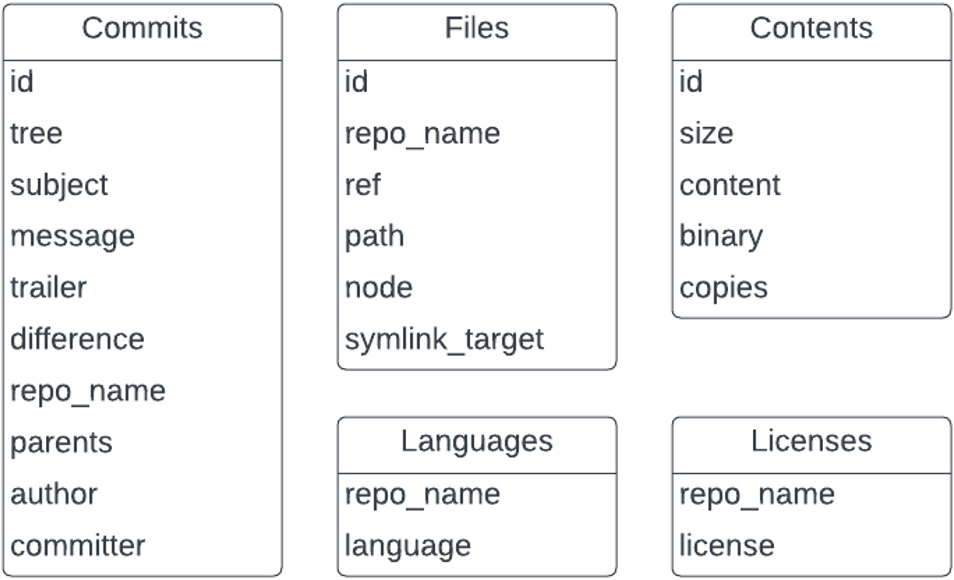
\includegraphics[width=0.7\textwidth]{./images/old_schema_BQ.png}
    \caption{BigQuery dataset's schema.}
    \label{image:db_schema}
\end{figure}

 Per poter lavorare in locale si è scelto di ridurre la dimensione del dataset ad un sample di $2000$ repository per un totale di $25.9$GB, inoltre, per arricchirne il valore dei dati, si è scelto di integrare i dati provenienti dall'API di GitHub.
In questo modo si riescono a sfruttare tre delle quattro "\textbf{V}" dei Big Data:
\begin{itemize}
    \item \textbf{Volume}: la quantità (in termini di volume) del sample estrapolato per le analisi permette di valutare le diverse soluzioni in termini di efficienza su un grande volume di dati.
    
    \item \textbf{Veracity}: essendo il dataset uno snapshot delle repository di GitHub, presenta informazioni veritiere riguardo ai commit e a tutti i dati associati. 

    \item \textbf{Variety}: i dati presi in considerazione provengono da due diverse fonti, Big Query e API di GitHub e si compongono di diverse srutture, rispettivamente: \textbf{JSON} e \textbf{CSV}.
\end{itemize}
Dallo schema precedentemente presentato è stato estratto il seguente grafo (vedi Fig.\ref{image:graph_schema}):
\begin{figure}[!ht]
    \centering
    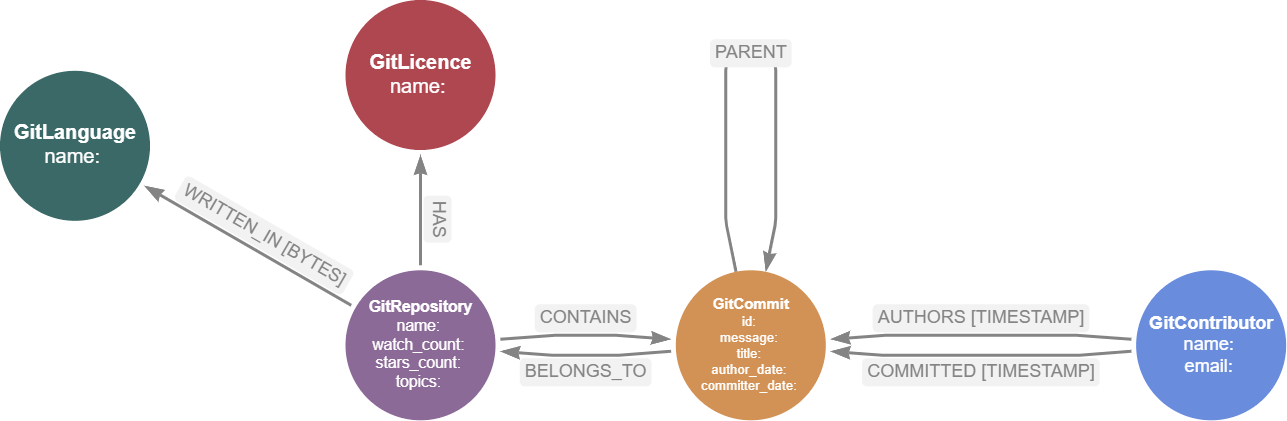
\includegraphics[width=\textwidth]{./images/graph_schema.png}
    \caption{Graph schema utilizzato per la comparazione delle soluzioni GDBMS sui dati estratti da GitHub.}
    \label{image:graph_schema}
\end{figure}

\newpage
\section{Architettura e Tecnologie}
Nella seguente sezione verranno presentate l'architettura e le tecnologie che sono state impiegate nello sviluppo del progetto.

\subsection{Architettura}
Per definire l'architettura del sistema è stato scelto \textbf{Docker Compose}, questo permette di strutturare applicazioni in grado di sostenere \textbf{scale-out} e \textbf{fault tolerance} con la possibilità di rilascio su cluster in poco tempo. L'architettura in questione viene presentata in Fig.\ref{image:docker_architecture}
\begin{figure}[!ht]
    \centering
    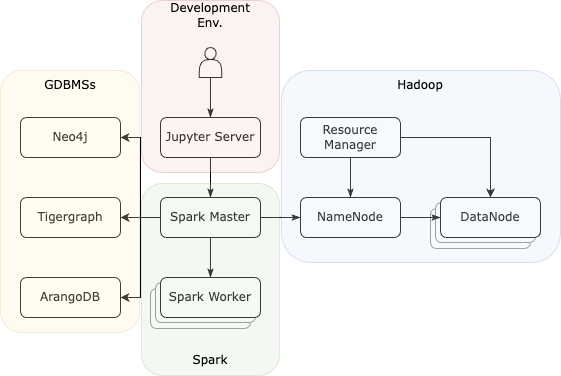
\includegraphics[width=.8\textwidth]{./images/ArchitetturaDocker.png}
    \caption{Servizi Docker.}
    \label{image:docker_architecture}
\end{figure}

Com'è possibile notare lo sviluppatore si interfaccia con con l'ambiente spark-hadoop tramite il server jupyter dal quale può lavorare sulle varie soluzioni GDBMS con i relativi connettori spark. Per sostenere scale-out è possibile incrementare il numero degli \codeinline{Spark Worker} e dei \codeinline{Data Node} per mezzo di file di configurazione, mentre, per sostenere fault tolerance è possibile incrementare il numero degli \codeinline{Spark Master} e dei \codeinline{Name Node}.

\begin{table}[!h]
\centering
\begin{tabular}{cc}
\toprule
Docker Image & Exposed Ports\\
\midrule
    namenode (hadoop) & 9870, 9000 \\
    datanode (hadoop) & - \\
    resourcemanager (hadoop) & - \\
    nodemanager1 (hadoop) & - \\
    historyserver (hadoop) & - \\
    spark-master & 8080, 7077 \\
    spark-worker & 8081 \\
    spark-history-server & 18081 \\
    jupyter-notebooks & 8888 \\
    neo4j & 7474, 7687 \\
    tigergraph & 14240 \\
    arangodb & 8529 \\
\bottomrule
\end{tabular}
\caption{Porte Docker aperte per l'architettura proposta.}
\label{tab:open_ports}
\end{table}

 Dunque, i dati nel sistema seguono il seguente flusso: una volta estratti da BigQuery, vengono immagazzinati su HDFS e arricchiti tramite l'API di GitHub per poi essere salvati su GDBMS. Una volta resi persistenti i dati vengono riletti per i task di analisi e visualizzazione.
\begin{figure}[!ht]
    \centering
    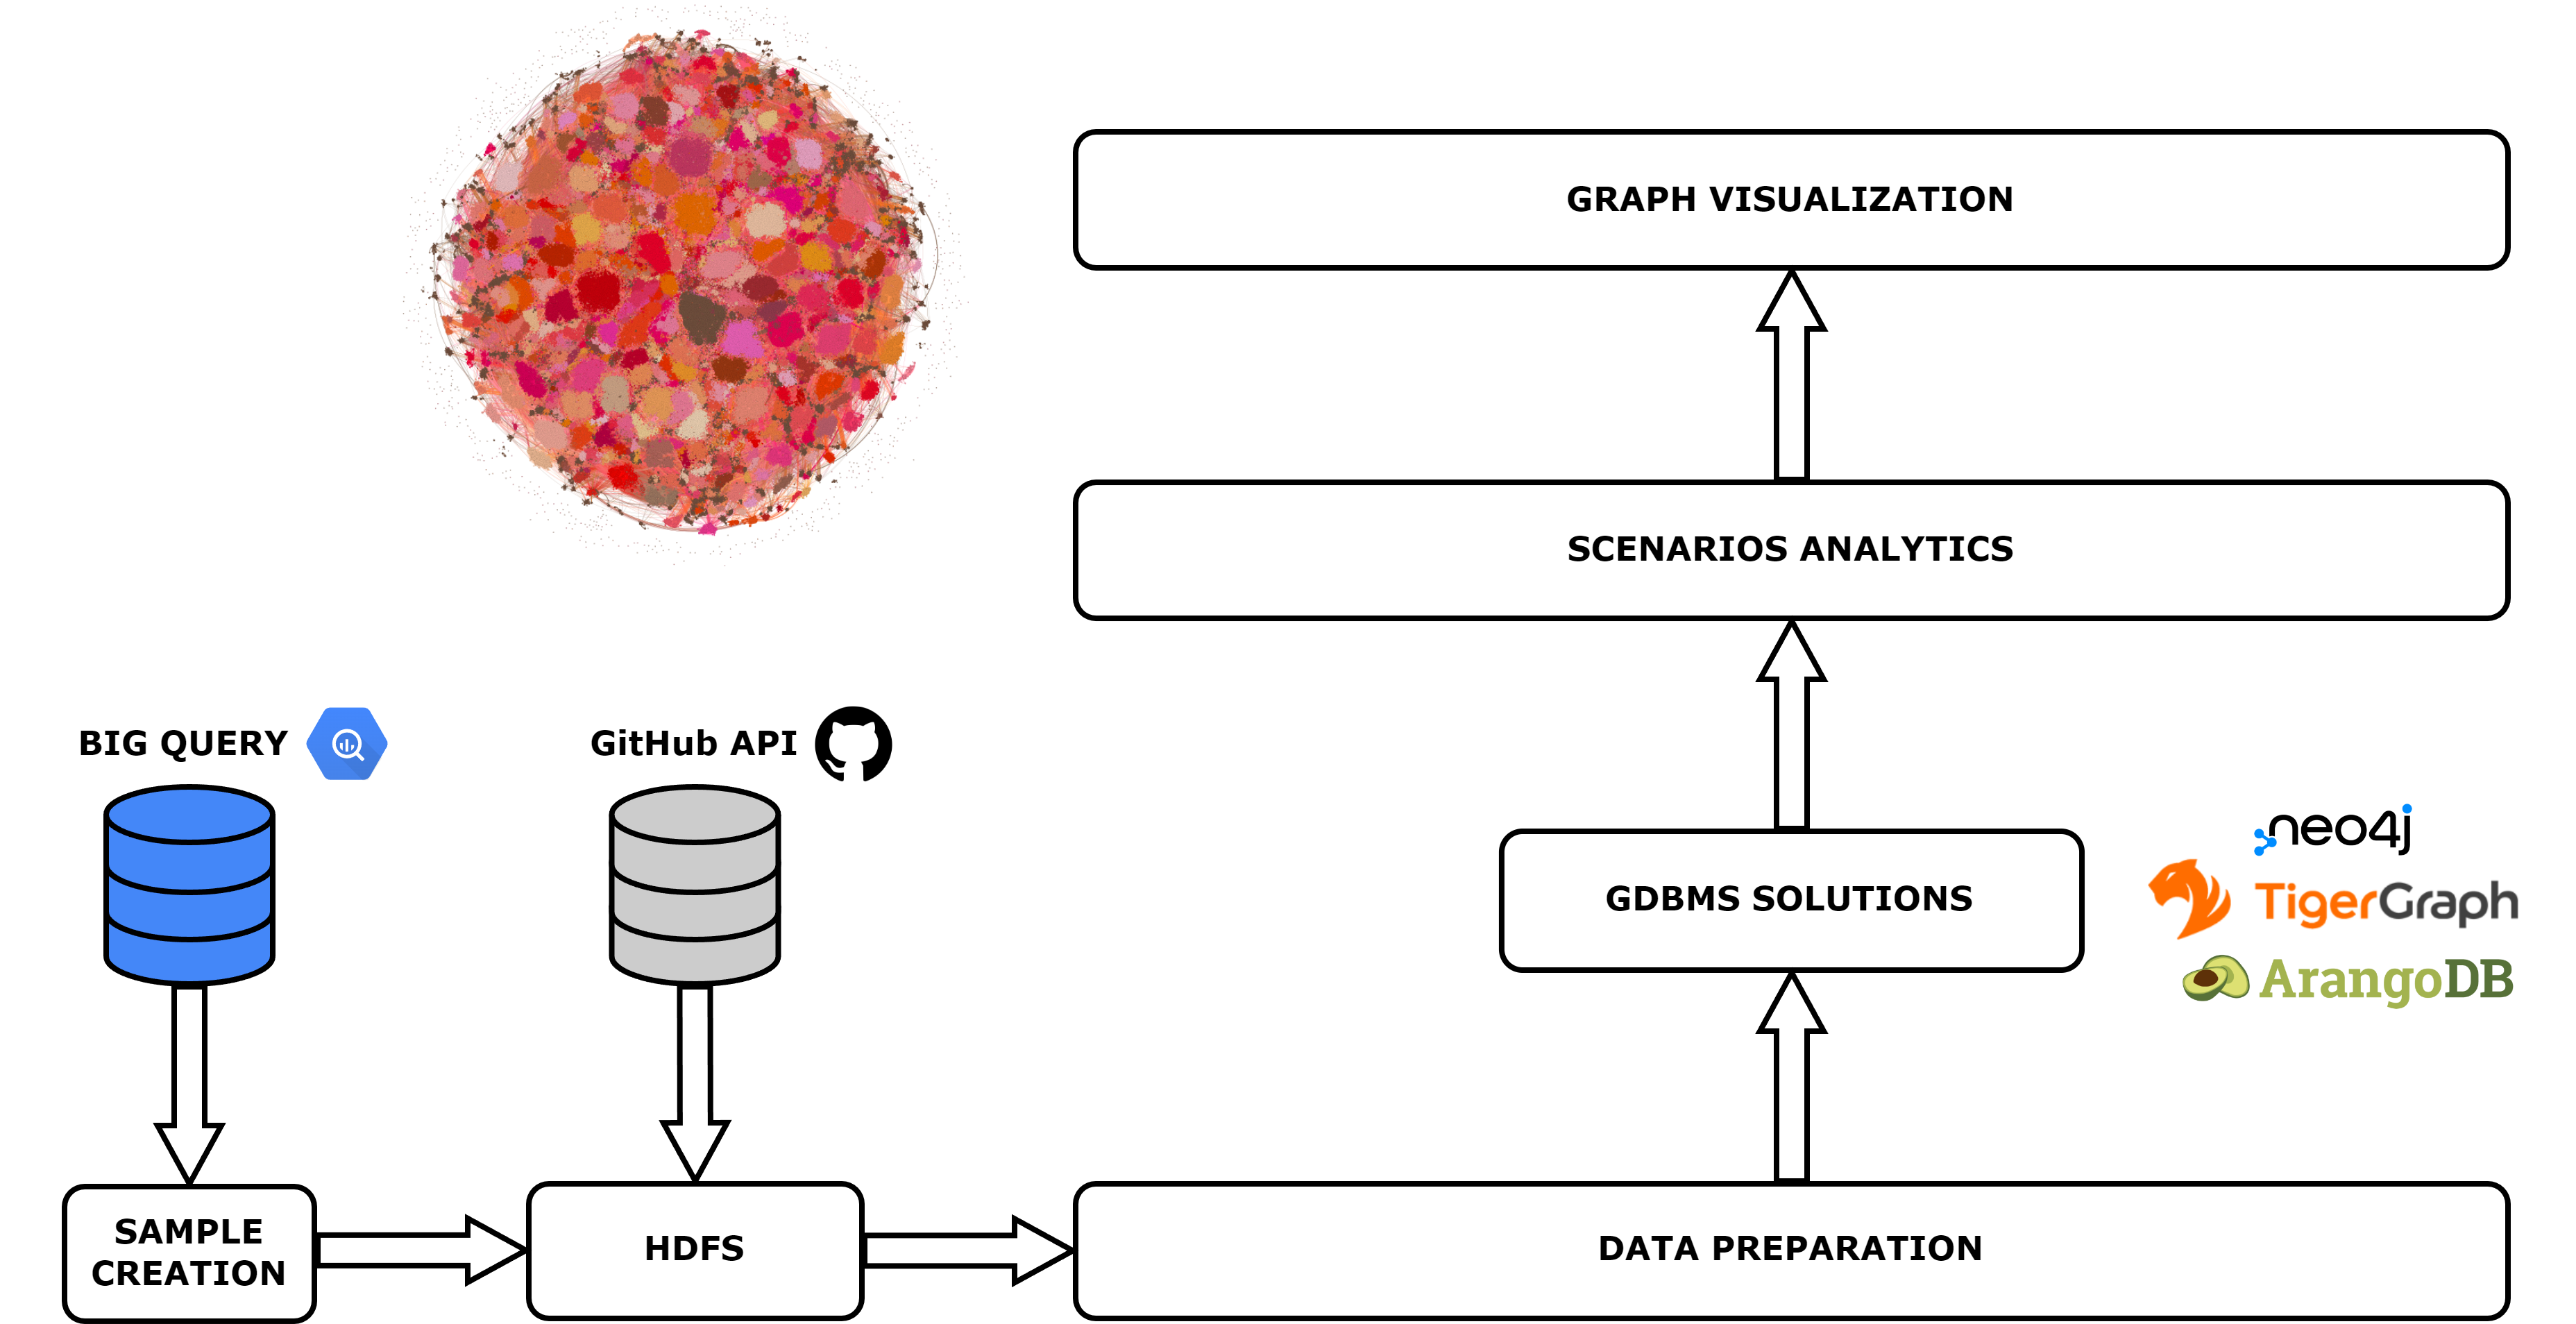
\includegraphics[width=\textwidth]{./images/architettura.png}
    \caption{Pipeline proposta per il confronto dei GDBMS.}
    \label{image:pipeline}
\end{figure}

\subsection{Tecnologie}
Di seguito sono riportate le tecnologie impiegate e le motivazioni dietro all'architettura proposta:
\begin{itemize}
    \item \textbf{Data Ingestion}: per questa fase sono stati utilizzati il query language di BigQuery e l'API python di GitHub;
    \item \textbf{Raw Layer}: per questo strato è stato scelto di utilizzare il file system distribuito di \textbf{Hadoop}, su cui è stato caricato il sample del dataset ottenuto dalla fase di Data Ingestion, proveniente dalle due pipeline rispettivamente di BQ e GitHub API.
    \item \textbf{Data Pre-Processing}: per il pre-processing del sample, visto il grande volume di dati da analizzare, è stato scelto di utilizzare \textbf{Spark}. La fase di pre-processing si compone in: una parte inziale di load dei dati dall'HDFS; successivamente viene fatta integrazione con le due fonti dati scelte; di seguito, vengono rimosse le ennuple duplicate e raffinato il campo testo per il campo chiave che contengono valori non ammessi dai db. Successivamente, avviene la creazione dei nodi e delle relazioni così come presenti in Fig.\ref{image:graph_schema}; e infine per ciascuna soluzione GDBMS tramite il connettore spark specifico i dati vengono caricati sul work layer.
    \item \textbf{Work Layer}: le soluzioni tecnlogiche di GDBMS scelte sono state \textbf{Neo4j}, \textbf{TigerGraph} e \textbf{ArangoDB} per la loro versatilità nel gestire grandi moli di dati ed essendo tra le uniche soluzioni free-to-use trovate per il caso d'uso.
    \item \textbf{Data Analytics}: le analisi effettuate sulle diverse soluzioni di GDBMS sono state composte di cinque scenari per testare l'efficienza in termini di tempi di risposta delle query e l'usabilità dei sistemi in generale (sia in termini di query language, essendo specifico per ogni soluzione, sia in termini di usabilità del connettore utilizzato). Inoltre, le analisi sono state estese anche a casi d'uso di Data Science valutandone le stesse metriche per questi task.
    \item \textbf{Data Visualization}: per la visualizzare del grafo, una volta popolato tramite i passi della pipeline precenti, è stato impiegato il tool \textbf{Gephi} specifico per la visualizzazione di large graphs.
\end{itemize}

 Per lavorare con i GDBMS è stato necessario l'utilizzo dei connettori spark di ciscuna implementazione. Per configurare spark in maniera tale de poter utilizzare questi connettori, oltre al download delle varie dipendenze, sono state scritte un insieme di funzioni che facilitano l'utilizzo di alcune impostazioni di default come le opzioni di connessione al server oppure le opzioni di lettura/scrittura salvate su un file di configurazione.

 Di seguito sono riportate quattro delle funzioni più utilizzate in  scrittura e lettura dei dati:
\begin{itemize}

    \item \codeinline{create_spark_session()} crea la sessione spark per effettuare scritture e letture su GDB sulla base del connettore spark \codeinline{connector}, dove \codeinline{dependencies} è il set delle dipendenze relative al connettore selezionato;

\begin{lstlisting}[style=PythonStyle, style=all]
def create_spark_session(app_name: str, connector: SparkConnector):
    build = SparkSession.builder.appName(app_name) \
        .master(SPARK_MASTER_URL)
    # Add the connector dependencies
    build = build.config("spark.jars", dependencies) \
        .config("spark.driver.extraClassPath", dependencies)
    return build.getOrCreate()
\end{lstlisting}
    
    \item \codeinline{get_default_options()}: riporta le opzioni comuni sia in fase di lettura che in fase di scrittura sulla base del parametro \codeinline{connector}, le quali sono presenti sul file di configurazione \codeinline{default-options.yaml};
\begin{lstlisting}[style=PythonStyle, style=all]
def get_default_options(connector: SparkConnector):
    options = {}
    for key in config[connector.value].keys():
        options[key] = config[connector.value][key]
    return options
\end{lstlisting}

\item \codeinline{spark_write()}: consente di scrivere un dataframe \codeinline{df} tramite un determinato connettore \codeinline{connector};
\begin{lstlisting}[style=PythonStyle, style=all]
def spark_write(connector: SparkConnector, df: DataFrame, mode: str, options: dict):
    # Get the connector format
    format = globals()[f"{connector.name}_FORMAT"]
    df.write.mode(mode) \
        .format(format) \
        .options(**options) \
        .save()
    print(f"Dataframe saved to {connector.name}")
\end{lstlisting}

    \item \codeinline{spark_read()}: consente di leggere i dati da un determinato GDBMS sulla base del connettore \codeinline{connector} e della sessione spark \codeinline{session}.
\begin{lstlisting}[style=PythonStyle, style=all]
def spark_read(connector: SparkConnector, session: SparkSession, options: dir) -> DataFrame:
    # Get the connector format
    format = globals()[f"{connector.name}_FORMAT"]
    df = session.read \
        .format(format) \
        .options(**options) \
        .load()
    print(f"Dataframe loaded from {connector.value}")
    return df
\end{lstlisting}
\end{itemize}

\section{GDBMS a Confronto}
Di seguito vengono illustrati gli scenari ideati per il confronto:
\begin{itemize}
    \item \textbf{Scenario 1}: individuare i contributori che hanno contribuito al maggior numero di repository (diverse);
    \item \textbf{Scenario 2}: individuare le repository che presentano codice in un determinato linguaggio per almeno una determinata soglia percentuale;
    \item \textbf{Scenario 3}: individuare il numero di commit di merge di una determinata repository;
    \item \textbf{Scenario 4}: individuare comunità all'interno del grafo per mezzo dell'algoritmo di \textbf{Label Propagation}; 
    \item \textbf{Scenario 5}: individuare i nodi più influenti nel grafo tramite l'algoritmo \textbf{PageRank}. 
\end{itemize}
\subsection{Configurazione Software/Hardware}
La configurazione con il quale sono stati effettuati i test è indicata di seguito in tab.\ref{tab:config_SWHW}:
\begin{table}[!h]
    \centering
    \begin{tabular}{|l|l|}
        \hline
        Processore & Intel(R) Core(TM) i7-9700 CPU @ 3.00GHz 3.00 GHz \\
        \hline
        RAM installata & 32,0 GB \\
        \hline
        Tipo sistema & Sistema operativo a 64 bit, processore basato su x64 \\
        \hline
    \end{tabular}
    \caption{Configurazione Software/Hardware impiegata per i test.}
    \label{tab:config_SWHW}
\end{table}



%%%%%%%%%%%%%%%%%
%% Neo4j %%%%%%%%
%%%%%%%%%%%%%%%%%
\subsection{Neo4j Implemented Scenarios}
Nella seguente sezione verranno illustrati gli scenari considerati per il GDBMS Neo4j. 
\begin{itemize}
    \item \textbf{Scenario 1}
\begin{lstlisting}[style = all, style = CypherStyle] 
MATCH (contrib:GitContributor)-[:AUTHOR]->
    (commit:GitCommit)-[:BELONGS_TO]->(repo:GitRepository) 
WITH contrib, COUNT(DISTINCT repo) AS repo_count
RETURN contrib, repo_count ORDER BY repo_count DESC
\end{lstlisting}

    \item \textbf{Scenario 2}
\begin{lstlisting}[style = all, style = CypherStyle] 
MATCH (r:GitRepository)-[w:WRITTED_IN]->(l:GitLanguage)
WITH r, SUM(w.bytes) AS totalBytesForRepo, collect({{language_name:l.name,bytes: w.bytes}}) AS bytesForLanguages
UNWIND bytesForLanguages AS bytesForLanguage
WITH r.name AS repo_name, bytesForLanguage.language_name AS lang, round((bytesForLanguage.bytes*1.0/totalBytesForRepo),2) AS percOfBytes
WHERE lang = "C++" AND percOfBytes > 0.5
RETURN repo_name, lang, percOfBytes 
\end{lstlisting}

    \item \textbf{Scenario 3}
\begin{lstlisting}[style = all, style = CypherStyle] 
MATCH (repository:GitRepository {{name: "tensorflow/tensorflow"}})<-[:BELONGS_TO]-(commit:GitCommit), r = (commit)-[:PARENT]->()
WITH commit, collect(r) AS parents
WHERE size(parents) > 1
RETURN count(commit) AS mergeCount
\end{lstlisting}
    
    \item \textbf{Scenario 4}
    \newline Per gli algoritmi di data science in neo4j è stato necessario definire una proiezione della porzione del grafo su cui si è voluto lanciare l'algoritmo e poi successivamente la query dell'algoritmo, di seguito il codice associato.

\begin{lstlisting}[style = all, style = CypherStyle] 
CALL gds.graph.project.cypher('contribRepoAndCommits',
'MATCH (n) WHERE n:GitContributor OR n:GitCommit OR         n:GitRepository RETURN ID(n) AS id',
'MATCH (n)-[r]->(m) WHERE r:PARENT OR r:BELONGS_TO OR       r:COMMITTED OR r:AUTHOR RETURN ID(n) AS source,         ID(m) AS target')
\end{lstlisting}

\begin{lstlisting}[style = all, style=CypherStyle] 
CALL gds.labelPropagation.stream('{PROJ_NAME}')
YIELD nodeId, communityId
RETURN nodeId AS ID, communityId AS community_id
ORDER BY community_id DESC
\end{lstlisting}

\item \textbf{Scenario 5}

Per lo scenario 5 è stata utilizzata la medesima proiezione del precente scenario, di seguito il codice associato alla chiamata dell'algoritmo.

\begin{lstlisting}[style = all, style=CypherStyle] 
CALL gds.pageRank.stream('contribRepoAndCommits')
YIELD nodeId, score
RETURN nodeId, score
ORDER BY score DESC
\end{lstlisting}
\end{itemize}


%%%%%%%%%%%%%%%%%
%% TigerGraph %%%
%%%%%%%%%%%%%%%%%
\subsection{TigerGraph Implemented Scenarios}
Nella seguente sezione verranno illustrati gli scenari considerati per il GDBMS TigerGraph. 
\begin{itemize}
    \item \textbf{Scenario 1}
\begin{lstlisting}[style = all, style=GSQLStyle] 
CREATE QUERY TopNAuthorsWithMoreContributes(INT N) FOR GRAPH Git
{
    TYPEDEF TUPLE<VERTEX<GitContributor> contributor, INT repo_count> Result_Tuple;
    MapAccum<VERTEX<GitContributor>, SetAccum<STRING>> @@contributors2repos;
    HeapAccum<Result_Tuple>(N, repo_count DESC) @@contributors2count;

    contributors = {GitContributor.*};

    p = SELECT con
        FROM contributors:con -(AUTHOR>:a)- GitCommit:com -(BELONGS_TO>:b)- GitRepository:repo
        ACCUM @@contributors2repos += (con -> repo.name);

    FOREACH (con, alist) IN @@contributors2repos DO
        @@contributors2count += Result_Tuple(con, alist.size());
    END;
  
    PRINT @@contributors2count;
}

INSTALL QUERY TopNAuthorsWithMoreContributes
RUN QUERY TopNAuthorsWithMoreContributes(10)
\end{lstlisting}

    \item \textbf{Scenario 2}
\begin{lstlisting}[style = all, style=GSQLStyle] 
CREATE QUERY ReposWithMoreThenPercentageOnLenguage(FLOAT perc, STRING lang) FOR GRAPH Git
{
    TYPEDEF TUPLE<VERTEX<GitRepository> repo, FLOAT percentage> Result_Tuple;
    MapAccum <VERTEX<GitRepository>, MapAccum<STRING, FLOAT>> @@repos2lang2bytesCount;
    ListAccum<Result_Tuple> @@result;

    repos = {GitRepository.*};
    s = SELECT r
        FROM repos:r -(WRITTEN_IN>:w)- GitLanguage:l
        ACCUM @@repos2lang2bytesCount += (r -> (l.name -> w.bytes));

    SumAccum<FLOAT> @@totalBytes;
    SumAccum<FLOAT> @@langBytes;
    FOREACH (r, lang2bytesCount) IN @@repos2lang2bytesCount DO
        @@totalBytes = 0.0;
        @@langBytes = 0.0;
        FOREACH (l, bytesCount) IN lang2bytesCount DO
            @@totalBytes += bytesCount;
            IF (lang == l) THEN
                @@langBytes = bytesCount;
            END;
        END;
        IF (lang2bytesCount.containsKey(lang) AND @@langBytes / @@totalBytes > perc) THEN
            @@result += Result_Tuple(r, @@langBytes / @@totalBytes);
        END;
    END;
    PRINT @@result;
}

INSTALL QUERY ReposWithMoreThenPercentageOnLenguage
RUN QUERY ReposWithMoreThenPercentageOnLenguage(0.5, "C++")
\end{lstlisting}
    \item \textbf{Scenario 3}
\begin{lstlisting}[style = all, style=GSQLStyle] 
CREATE QUERY CountMergeCommits(STRING repo_name) FOR GRAPH Git
{
    TYPEDEF TUPLE<INT mergeCount> Result_Tuple;
    SumAccum<INT> @parentsCount;
    ListAccum<VERTEX<GitCommit>> @@mergeCommitsList;
    repos = {GitRepository.*};
    commits = {GitCommit.*};

    selectedRepo =  
            SELECT r 
            FROM repos:r 
            WHERE r.name == repo_name;

    selectedCommits =   
            SELECT comm
            FROM selectedRepo:repo -(CONTAINS>)- commits:comm -(PARENT>)- GitCommit:parent
            ACCUM comm.@parentsCount += 1;

    mergeCommits = 
            SELECT comm
            FROM selectedCommits:comm
            WHERE comm.@parentsCount > 1
            ACCUM  @@mergeCommitsList += comm;
  
    PRINT @@mergeCommitsList.size() AS mergeCount;
}

INSTALL QUERY CountMergeCommits
RUN QUERY CountMergeCommits("tensorflow/tensorflow")
\end{lstlisting}
    \item \textbf{Scenario 4}
\begin{lstlisting}[style = all, style=GSQLStyle] 
RUN QUERY tg_label_prop( ["GitContributor", "GitRepository", "GitCommit"],  ["CONTAINS", "PARENT", "BELONGS_TO", "AUTHOR", "COMMITTED"], 250, -1, _, _, _)
\end{lstlisting}

    \item \textbf{Scenario 5}
\begin{lstlisting}[style = all, style=GSQLStyle] 
RUN QUERY tg_pagerank(["GitContributor", "GitRepository", "GitCommit"], ["CONTAINS", "PARENT", "BELONGS_TO", "AUTHOR", "COMMITTED"], 0.001, 25, 0.85, 10, _, _, _, _)
\end{lstlisting}
\end{itemize}


%%%%%%%%%%%%%%%%%
%% ArangoDB %%%%%
%%%%%%%%%%%%%%%%%

\newpage
\subsection{ArangoDB Implemented Scenarios}
Nella seguente sezione verranno illustrati gli scenari considerati per il GDBMS ArangoDB. 
\begin{itemize}
    \item \textbf{Scenario 1}
    \begin{lstlisting}[style = all, style = ArangoStyle] 
LET distinctValues = (
    FOR c IN GitContributor
        FOR commit IN OUTBOUND c AUTHOR
            FOR r IN OUTBOUND commit BELONGS_TO
                RETURN DISTINCT{c, r}
)
FOR d IN distinctValues
    COLLECT contrib = d.c.name WITH COUNT INTO repo_count
    SORT repo_count DESC
    FILTER repo_count > 1
    LIMIT 10
    RETURN {contrib, repo_count}
    \end{lstlisting}

    \item \textbf{Scenario 2}
    \begin{lstlisting}[style = all, style = ArangoStyle] 
FOR repo IN GitRepository
    LET repoTotalBytes = (
    FOR lan IN OUTBOUND repo WRITTEN_IN
        LET byteInfo = (
            FOR info IN WRITTEN_IN
            FILTER info._from==repo._id AND 
                   info._to==lan._id
            RETURN info.bytes)
        COLLECT repository = repo._key
        AGGREGATE repoTotalBytes = SUM(byteInfo[0])
        RETURN {repository, repoTotalBytes}
        )
    
    FILTER LENGTH(repoTotalBytes) > 0 
    
    FOR lan IN OUTBOUND repo WRITTEN_IN
        LET byteInfo = (
          FOR info IN WRITTEN_IN
            FILTER info._from==repo._id AND 
                   info._to==lan._id
            RETURN info.bytes
            )
        COLLECT repo_name=repo._key, language=lan._key, percentageOfBytes=(byteInfo[0]/repoTotalBytes[0].repoTotalBytes)
        FILTER language=="Cpp" AND percentageOfBytes>0.5
        RETURN {
          repo_name, 
          language,
          percentageOfBytes
          }
    \end{lstlisting}
    \newpage
    \item \textbf{Scenario 3}
    \begin{lstlisting}[style = all, style = ArangoStyle] 
FOR repo IN GitRepository
    FILTER repo._key == "tensorflow::tensorflow"
    FOR commit IN INBOUND repo BELONGS_TO
    LET parents = ( 
        FOR parent IN OUTBOUND commit PARENT
            COLLECT comm = commit._key INTO parents
            RETURN {lun: length(parents), comm}
            )
    FILTER parents[0].lun>1 AND 
           parents[0].comm == commit._key
    COLLECT WITH COUNT INTO n_merge
    RETURN {num_merge: n_merge}
\end{lstlisting}

\item \textbf{Scenario 4}
    \begin{lstlisting}[style = all, style = PythonStyle] 
# Start a new Pregel job in "github_graph".
job_id = db.pregel.create_job(
    graph='github_graph',
    algorithm='labelpropagation',
    store=False,
    max_gss=250,
    thread_count=1,
    async_mode=False,
    result_field='community'
)

# Retrieve details of a Pregel job by ID.
job = pregel.job(job_id)
\end{lstlisting}

\begin{lstlisting}[style = all, style = ArangoStyle] 
FOR v IN PREGEL_RESULT({job["id"]})
RETURN {{key: v._key, rank: v.result}}
\end{lstlisting}

\item \textbf{Scenario 5}
    \begin{lstlisting}[style = all, style = PythonStyle] 
# Start a new Pregel job in "github_graph".
job_id = db.pregel.create_job(
    graph='github_graph',
    algorithm='pagerank',
    store=False,
    max_gss=250,
    thread_count=1,
    async_mode=False,
    result_field='result',
    algorithm_params={'threshold': 0.000001}
)

# Retrieve details of a Pregel job by ID.
job = pregel.job(job_id)
\end{lstlisting}

\begin{lstlisting}[style = all, style = ArangoStyle] 
FOR v IN PREGEL_RESULT({job["id"]})
RETURN {key: v._key, community: v.community}
\end{lstlisting}

\end{itemize}

%%%%%%%%%%%%%%%%%%%%%%%%%%%%%%%%%%%%%%%%%%%%%%%%%%%%%%%%%%%%%%%
%assegnare le label del linguaggio alle repo, sulla base dei bytes, e predire se il testo del commit è assegnato alla label della repo. (si può fare anche con scala continua)
%%%%%%%%%%%%%%%%%%%%%%%%%%%%%%%%%%%%%%%%%%%%%%%%%%%%%%%%%%%%%%

\subsection{Risultati Ottenuti e Confronti Effettuati}
Per il confronto dei risultati sono stati effettuati i test con subset del dataset a grandezza crescende, così da poter osservare il comportamento dei diversi GDBMS e le loro prestazioni in termini di tempo. Inoltre, verranno elencate le differenze nei Query Languages in termini di usabilità.

\subsubsection{Output}
Nella seguente sezione verranno riportati le prime 10 rows degli output (essendo corretti e uguali per tutte le soluzioni GDBMS adottate per il confronto, verrannno tabellati solo un unico output per ciascuno scenario) degli scenari ideati per il confronto, per farne capire meglio la logica. 
\begin{itemize}
    \item \textbf{Scenario 1}

    
\begin{table}[!ht]
    \centering
    \begin{tabular}{cc}
    \toprule
    Contributor name & Repo Count \\
    \midrule
    dependabot[bot] & 293 \\
    The Gitter Badger & 138 \\
    Prayag Verma & 128 \\
    ReadmeCritic & 117 \\
    Ikko Ashimine & 96 \\
    Tim Gates & 90 \\
    Kevin Kirsche & 62 \\
    Greenkeeper & 57 \\
    Morton Fox & 57 \\
    Andrew Murray & 54 \\
    \bottomrule
    \end{tabular}
\end{table}



    \item \textbf{Scenario 2}

\begin{table}[!ht]
    \centering
    \begin{tabular}{ccc}
    \toprule
    Language & Percentage Of Bytes & Repo Name\\
    \midrule
    C++ & 0.65 & grpc/grpc\\
    C++ & 0.58 & ValveSoftware/openvr\\
    C++ & 0.88 & godotengine/godot\\
    C++ & 0.63 & tensorflow/tensorflow\\
    C++ & 0.67 & mobile-shell/mosh\\
    C++ & 0.97 & nlohmann/json\\
    C++ & 0.9 & google/googletest\\
    C++ & 0.9 & google/ion\\
    C++ & 0.88 & koekeishiya/kwm\\
    C++ & 0.6 & swoole/swoole-src\\
    \bottomrule
    \end{tabular}
\end{table}


    \item \textbf{Scenario 3}

    \begin{table}[!ht]
        \centering
        \begin{tabular}{cc}
        \toprule
        Repo Name & Merge Number \\
        \midrule
            tensorflow/tensorflow & 12127 \\
        \bottomrule
        \end{tabular}
    \end{table}

    \newpage
    \item \textbf{Scenario 4}

Per quanto riguarda lo scenario 4 le comunità identificate dall'algoritmo di Label Propagation sulla proiezione del grafo con i nodi GitRepository, GitCommit e GitContributor sono le seguenti (per la visualizzazione su Gephi è stato utilizzato l'algoritmo di visualizzazione \textbf{OpenOrd} e all'aumentare del numero delle repositories, rispettivamente: 10, 100, 1000, 2000 repos):

\begin{figure}[!ht]
    \centering
    \begin{subfigure}{.5\textwidth}
        \centering
        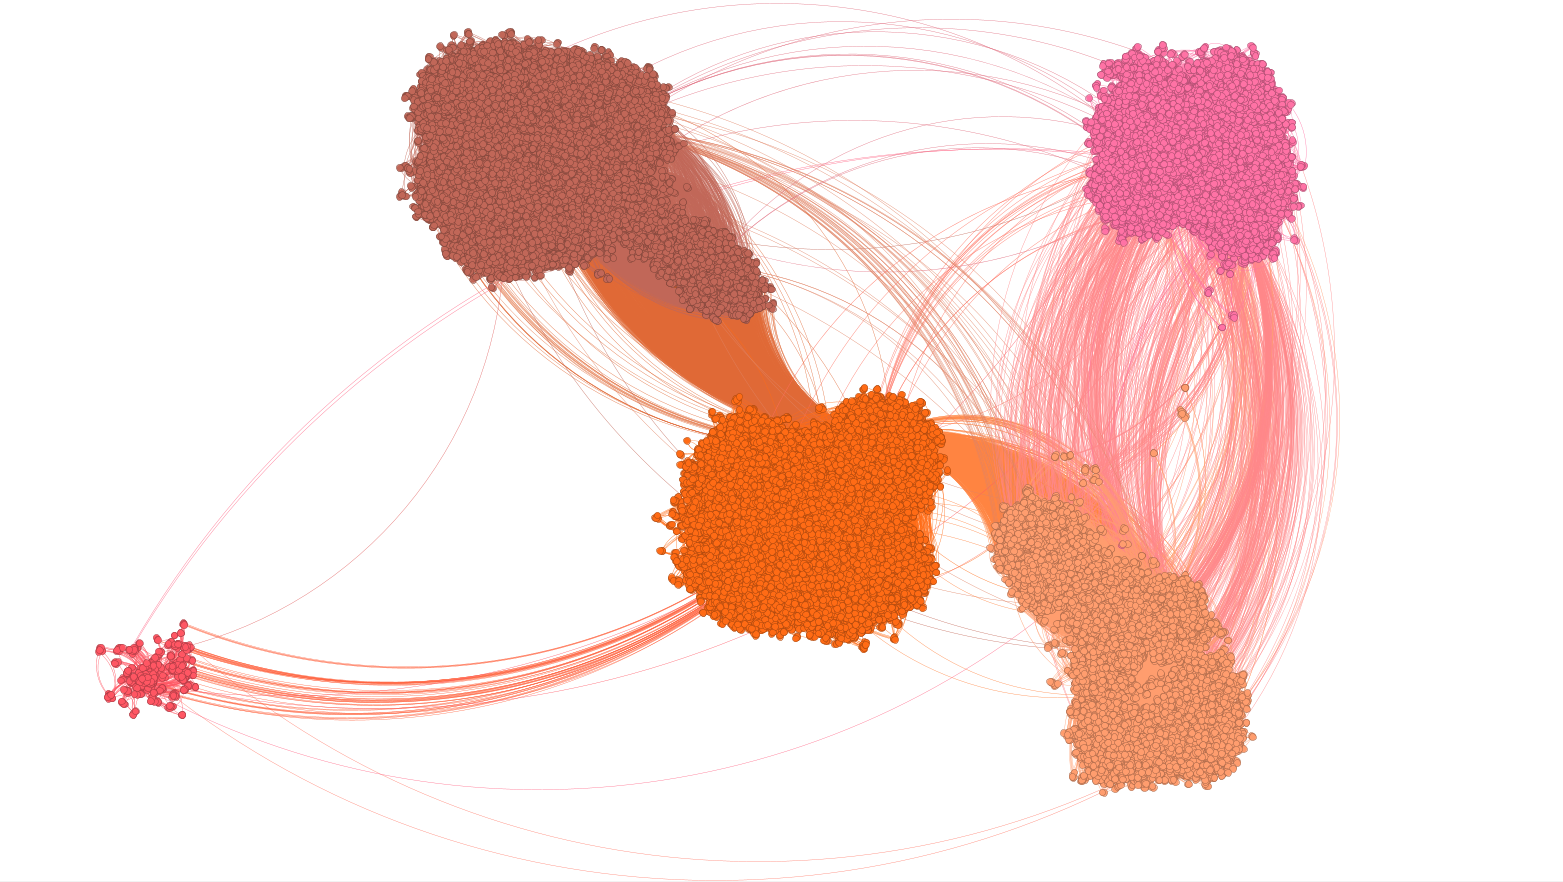
\includegraphics[width=\linewidth]{./images/OpenOrdLabelProp_10.png}
        \caption{Label Propagation con 10 repositories.}
        \label{fig:LabelPropagation10}
    \end{subfigure}%
    \begin{subfigure}{.5\textwidth}
        \centering
        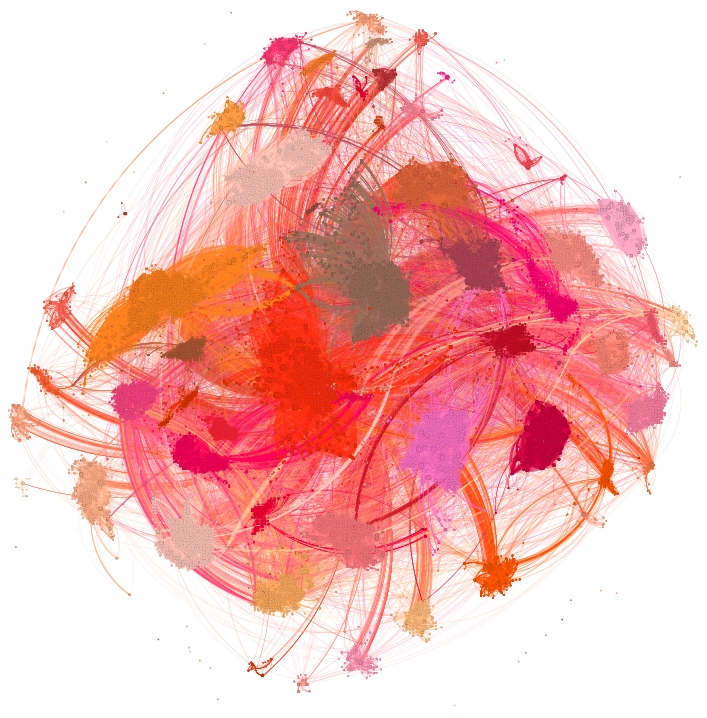
\includegraphics[width=\linewidth]{./images/OpenOrdLabelProp_100.png}
        \caption{Label Propagation con 100 repositories.}
        \label{fig:LabelPropagation100}
    \end{subfigure}\\[1ex] % Aggiunto uno spazio verticale tra le due coppie di immagini
    \begin{subfigure}{.5\textwidth}
        \centering
        
\includegraphics[width=\linewidth]{./images/OpenOrdLabelProp_1000.png}
        \caption{Label Propagation con 1000 repositories.}
        \label{fig:LabelPropagation1000}
    \end{subfigure}%
    \begin{subfigure}{.5\textwidth}
        \centering
        
\includegraphics[width=\linewidth]{./images/OpenOrdLabelProp_2000.png}
        \caption{Label Propagation con 2000 repositories.}
    \end{subfigure}
    \caption{Label Propagation all'aumentare del numero delle repositories.}
    \label{fig:TutteLeConfigurazioni}
\end{figure}

Si può notare in fig.\ref{fig:TutteLeConfigurazioni} che, tramite l'algoritmo di Label Propagation sono state identificate comunità che racchiudono le repo, i loro commit e contributori associati.

    \newpage
    \item \textbf{Scenario 5}

\begin{table}[!ht]
    \centering
    \begin{tabular}{cc}
    \toprule
    Repo Name & Score \\
    \midrule
    tensorflow/tensorflow & 15630.063491839835 \\
    apple/swift & 15427.057959425001 \\
    kubernetes/kubernetes & 12170.155320558157 \\
    dotnet/roslyn & 10044.6008681273 \\
    Microsoft/vscode & 9750.781070613648 \\
    rails/rails & 9693.129889366524 \\
    Homebrew/homebrew & 7593.8009527367085 \\
    symfony/symfony & 6869.918907495444 \\
    ansible/ansible & 6393.512080307458 \\
    golang/go & 6262.886339651076 \\
    \bottomrule
    \end{tabular}
\end{table}    
\end{itemize}

\subsubsection{Caratteristiche e Usabilità}
Di seguito sono riportate alcune osservazioni sull'usabiulià delle tre soluzioni:
\begin{itemize}
    \item \textbf{Neo4j}: un query language estremamente intuitivo che segue il flusso di dati a grafo con costrutti come arco (->) e nodo, una buona documentazione, la presenza di molto materiale in rete e la semplicità di configurazione del connettore spark fanno si che neo4j abbia un'alta usabilità; 
    \item \textbf{TigerGraph}: il query language prolisso ed il fatto che per poter eseguire una query questa deve essere installata, una buona documentazione, poco materiale in rete e la semplicità di configurazione fanno si che tigergraph abbia una non molto buona usabilità;
    \item \textbf{ArangoDB}: infine, il query language di arangoDB è stato concepito per lavorare bene su più data model, il che rende la formazione della query su grafo meno intuitiva di Neo4j. Inoltre presenta un numero più ridotto di algoritmi di data science (ad esempio il noto algoritmo di Louvain per l'dentificazione delle comunità) rispetto alle altre due soluzioni impiegate. Il tutto rende la sua usabilità nella media.
\end{itemize}
In Tab.\ref{tab:features_GDBMS} e Tab.\ref{tab:query_langugaes} vengono riassunte, rispettivamente, le caratteristiche osservate dei GDBMS considerati per le analisi e le differenze nei diversi query language.
\begin{table}[!ht]
\centering

\begin{tabular}{cccc}
\toprule
Features & Neo4j & Tigergraph & ArangoDB \\
\midrule
    Architecture & Single server & Single server & Single server \\
    Language & Cypher & GSQL & AQL \\
    Written in & Java & C++ & C++ \\
    Protocols & Bolt & Http & Http \\
    Algo-Computation-availability & High & High & Medium \\
    Data model & Graph & Graph & Document, graph, key-value \\
    Schema free & Yes & No & Yes \\
\bottomrule
\end{tabular}
\caption{Features of the GDBMS considered.}
\label{tab:features_GDBMS}
\end{table}


\begin{table}[!ht]
\centering
\begin{tabular}{cccc}
\toprule
Features & Cypher & GSQL & AQL \\
\midrule
Effort (Query formation) & Low & High & Medium \\
Readability & High & Medium & Medium \\
%Example query & - & - & - \\
\bottomrule
\end{tabular}
\caption{Features of Query Language of the GDBMS considered.}
\label{tab:query_langugaes}
\end{table}
% da inserire in tabella
%% CREATE QUERY CommitRepos(STRING repo_name) FOR GRAPH Git
%{
%    repos = {GitRepository.};
%    commits = {GitCommit.};
%    selectedRepo = SELECT r FROM repos:r WHERE r.name == repo_name;
%
%    selectedCommits = SELECT comm FROM selectedRepo:repo -(CONTAINS>)- commits:comm;
%}

\newpage
\subsubsection{Prestazioni}
In questa sezione vengono riportati i tempi di lettura da HDFS, scrittura su GDBMS ed i tempi di elaborazione dei vari scenari all'aumentare del volume dei dati. Per simulare l'incremento del volume è stato scelto di dividere il dataset in campioni di dimensioni ridotte come riportato di seguito in Tab.\ref{tab:sample_dim}. Inoltre, i tempi ottenuti dai test sono stati graficati (su scala logaritmica) per effettuarne il confronto.

\begin{table}[h]
    \centering
    \begin{tabular}{lcccc}
    \toprule
    \textbf{\#Repository} & \textbf{Nodi} & \textbf{Relazioni} & \textbf{Dimensione} \\
    \midrule
        \textbf{10} & 225 K  & 865 K  & 1.68 GB \\
        \textbf{100}  & 910 K  & 3.6 M  & 4.85 GB \\
        \textbf{1000} & 3.6 M  & 14.5 M & 20.8 GB \\
        \textbf{2000} & 5.23 M & 20.9 M & 25.9 GB \\
    \bottomrule
    \end{tabular}
    \caption{Dimensioni dei sample utilizzati per i confronti.}
    \label{tab:sample_dim}
\end{table}

\begin{itemize}
    \item \textbf{Writing Time}:
    \begin{figure}[!ht]
        \centering
        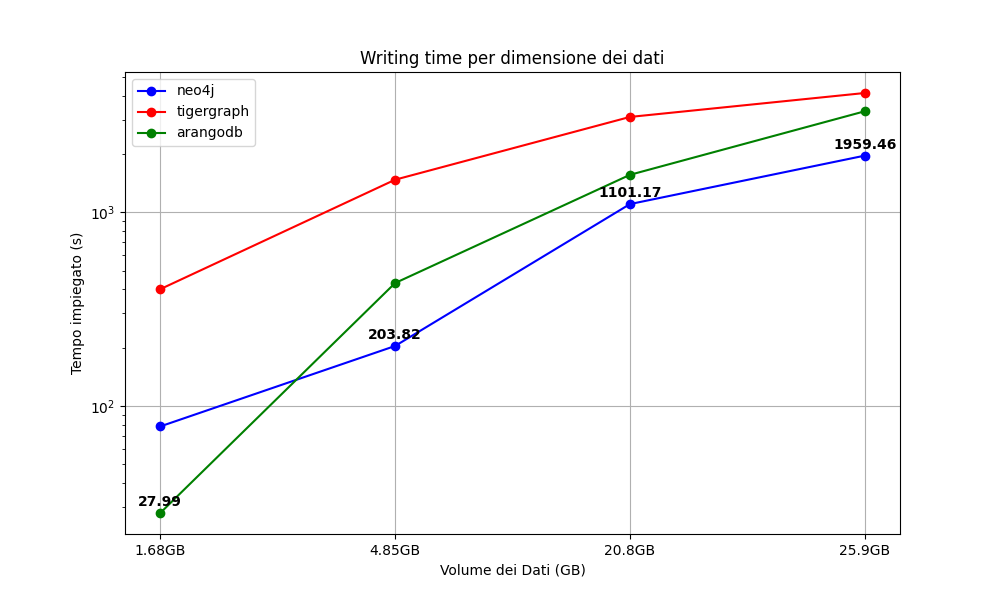
\includegraphics[width=\textwidth]{./images/plot_results/wtime.png}
    \end{figure}

    \newpage
    \item \textbf{Scenario 1}:
    \begin{figure}[!ht]
        \centering
        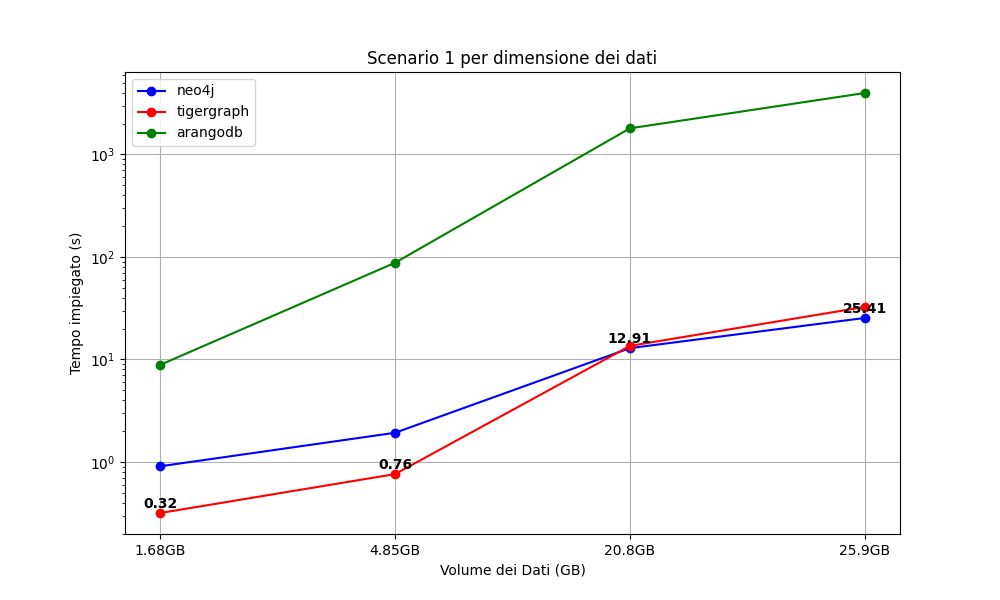
\includegraphics[width=\textwidth]{./images/plot_results/scenario1.png}
    \end{figure}

    \item \textbf{Scenario 2}:
    \begin{figure}[!ht]
        \centering
        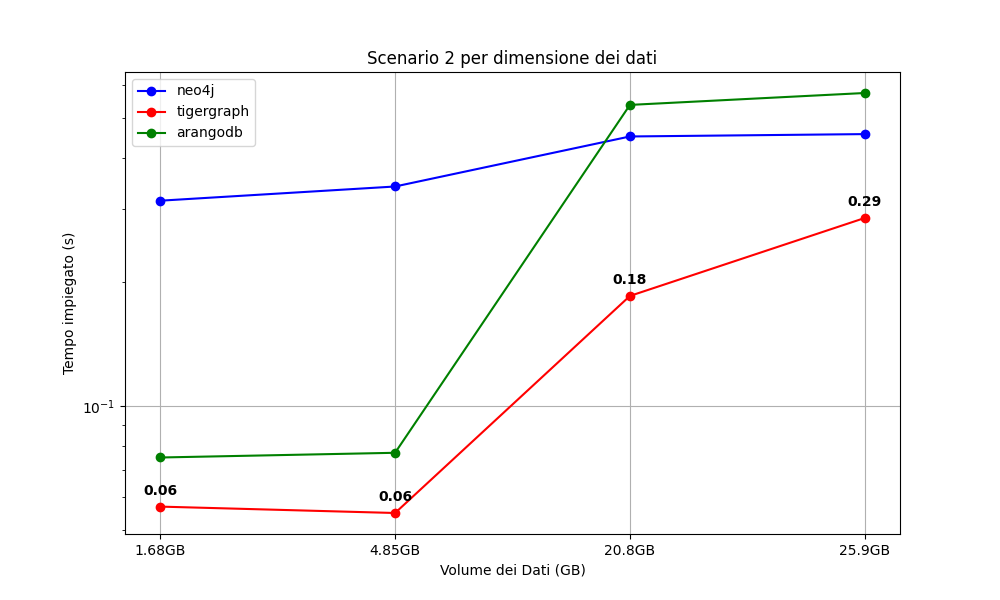
\includegraphics[width=\textwidth]{./images/plot_results/scenario2.png}
    \end{figure}

    \newpage
    \item \textbf{Scenario 3}:
    \begin{figure}[!ht]
        \centering
        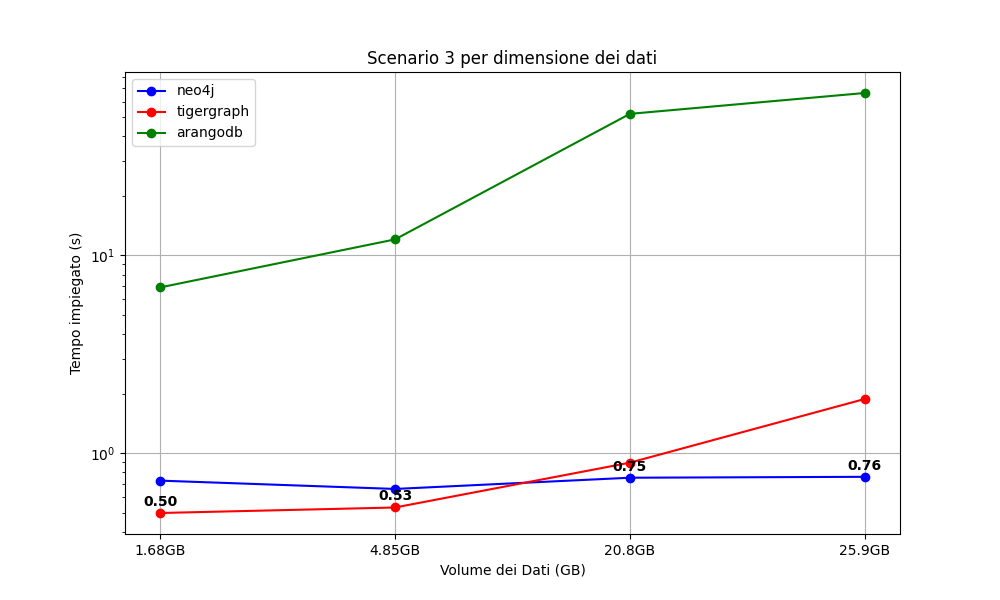
\includegraphics[width=\textwidth]{./images/plot_results/scenario3.png}
    \end{figure}

    
    \item \textbf{Scenario 4}:
    \begin{figure}[!ht]
        \centering
        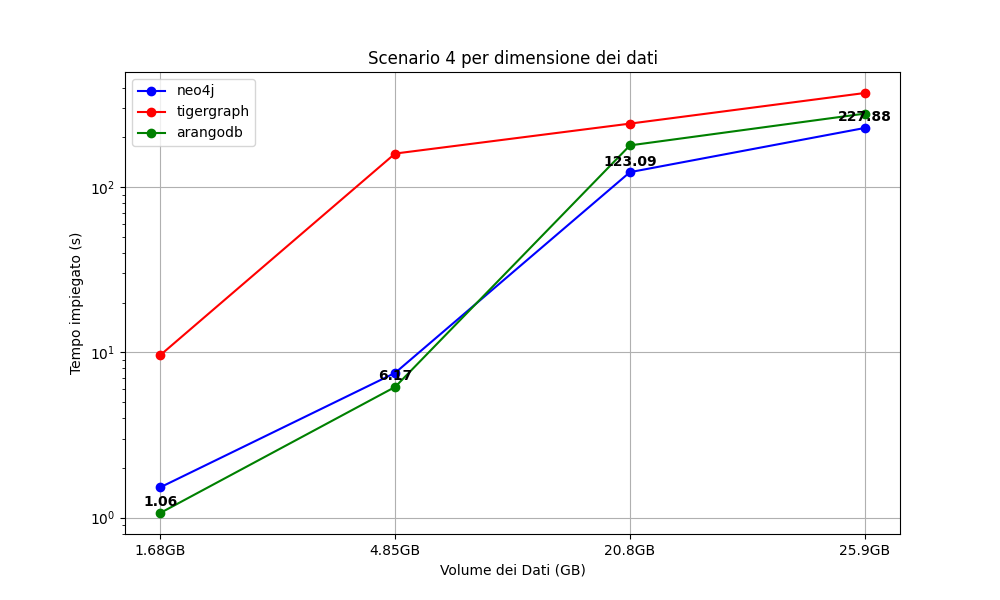
\includegraphics[width=\textwidth]{./images/plot_results/scenario4.png}
    \end{figure}

    \newpage
    \item \textbf{Scenario 5}:
    \begin{figure}[!ht]
        \centering
        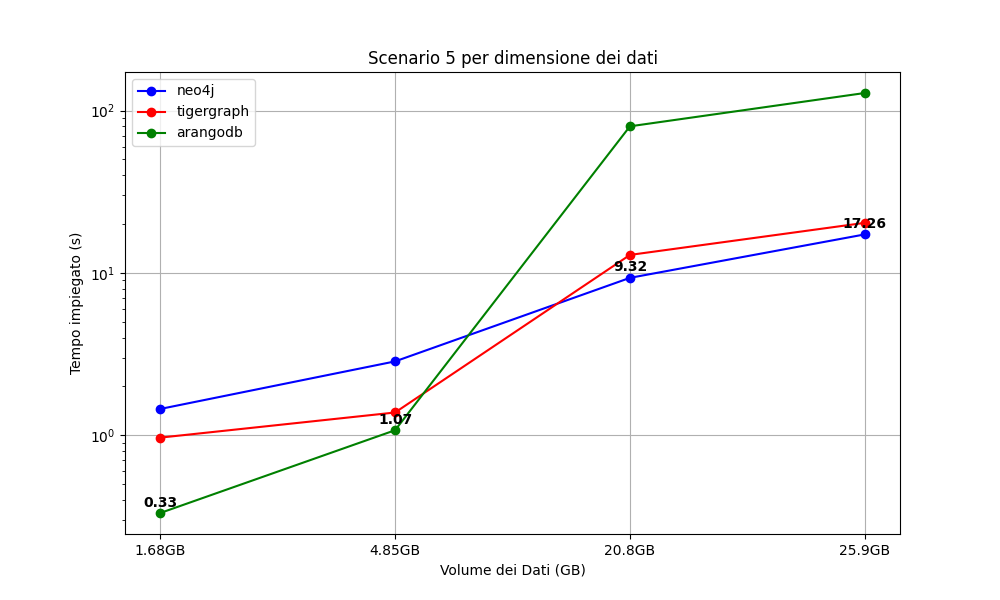
\includegraphics[width=\textwidth]{./images/plot_results/scenario5.png}
    \end{figure}
    
\end{itemize}

\section{Conclusioni}
Analizzando i risultati ottenuti, si è potuto osservare che in termini di usabilità, nelle tre soluzioni identificate, Neo4j è quello che ne possiede la migliore ed è sicuramente la scelta più adatta per uno sviluppatore che si affaccia per la prima volta ai Graph DB. ArangoDB è un po meno utilizzabile di Neo4j principalmente a causa della sua versatilità su diversi data model. Infine, Tigergraph è sicuramente il più completo fra i tre, anche in termini di algoritmi di presenti per la data analytics, ma comunque presenta un query language molto complesso per chi si affaccia per la prima volta al mondo dei Graph DB prestandosi bene ad un developer più esperto.
\newline Per quanto riguarda invece le prestazioni, dai risultati ottenuti, si può vedere che Neo4j performa meglio in scrittura e si comporta in media bene su tutti gli scenari (in particolare nello scenario 3, dove riesce a mantenere un tempo di esecuzione quasi costante all'aumentare del valume del dataset). Successivamente, viene TigerGraph che ha il tempo di scrittura più alto fra le tre soluzioni ma che ottiene i risultati migliori per primo e secondo scenario, si comporta nella media con l'algoritmo PageRank e male, essendo la soluzione peggiore, per quanto riguarda Louvain. Infine, per ArangoDB i tempi di scrittura sono di poco peggiori rispetto a quelli di Neo4j, lo schema d'esecuzione per le subquery definite nello scenario 1 e 3 che utilizza la \codeinline{COLLECT WITH COUNT}\footnote{\href{https://www.arangodb.com/learn/documents/making-subqueries-fast/}{ArangoDB official article for not optimized query COLLECT WITH COUNT with subqueries.}} non è particolarmente ottimizzato internamente dal db e performa decisamente peggio delle altre soluzioni, per lo scenario 4 invece le prestazioni sono simili a quelle di Neo4j e per lo scenario 5 infine scala male all'aumentare del volume di dati. \newline
Per cui in conclusione si può dire che per le scritture performa meglio Neo4j, la scelta migliore per task di graph traversal classici (dall'1 al 3 scenario) ricadrebbe su TigerGraph e per task di Data Analytics (4 e 5 scenario)     invece Neo4j. 


\end{document}
